%%% License: Creative Commons Attribution Share Alike 4.0 (see https://creativecommons.org/licenses/by-sa/4.0/)

\documentclass[english,10pt
,aspectratio=169
%,handout
%,notes
]{beamer}
%%% License: Creative Commons Attribution Share Alike 4.0 (see https://creativecommons.org/licenses/by-sa/4.0/)

\DeclareGraphicsExtensions{.eps, .pdf,.png,.jpg,.mps,}
\usetheme{reMedian}
\usepackage{parskip}
\makeatother

\renewcommand{\baselinestretch}{1.1} 

\usepackage{amsmath, amssymb, amsfonts, amsthm}
\usepackage{enumerate}
%\usepackage{enumitem}
\usepackage{hyperref}
\usepackage{url}
\usepackage{bbm}
\usepackage{color}

\usepackage{tikz}
\usepackage{tikzscale}
%\newcommand*\circled[1]{\tikz[baseline=(char.base)]{
%		\node[shape=circle,draw, inner sep=-20pt] (char) {#1};}}
%\usetikzlibrary{automata,positioning}
%\usetikzlibrary{decorations.pathreplacing}
\usepackage{pgfplots}
\usepgfplotslibrary{fillbetween}
\usepackage{graphicx}

\usepackage{setspace}
%\thinmuskip=1mu
%\medmuskip=1mu 
%\thickmuskip=1mu 


%\usecolortheme{default}
\usepackage{verbatim}
\usepackage[normalem]{ulem}

\usepackage{apptools}
\AtAppendix{
	\setbeamertemplate{frame numbering}[none]
}
\usepackage{natbib}


% red strikeout
\newcommand\soutred{\bgroup\markoverwith
	{\textcolor{red}{\rule[0.55ex]{2pt}{0.8pt}}}\ULon}



%% To use LyX frames from old version:
%\def\lyxframeend{} % In case there is a superfluous frame end
%\long\def\lyxframe#1{\@lyxframe#1\@lyxframestop}%
%\def\@lyxframe{\@ifnextchar<{\@@lyxframe}{\@@lyxframe<*>}}%
%\def\@@lyxframe<#1>{\@ifnextchar[{\@@@lyxframe<#1>}{\@@@lyxframe<#1>[]}}
%\def\@@@lyxframe<#1>[{\@ifnextchar<{\@@@@@lyxframe<#1>[}{\@@@@lyxframe<#1>[<*>][}}
%\def\@@@@@lyxframe<#1>[#2]{\@ifnextchar[{\@@@@lyxframe<#1>[#2]}{\@@@@lyxframe<#1>[#2][]}}
%\long\def\@@@@lyxframe<#1>[#2][#3]#4\@lyxframestop#5\lyxframeend{%
%	\frame<#1>[#2][#3]{\frametitle{#4}#5}}


\title{Mechanism Design}

\subtitle{8: Communication with verifiable information}

\author{Egor Starkov}

\date{K{\o}benhavns Unversitet \\
	Fall 2022}


\begin{document}
	\AtBeginSection[]{
		\frame{
			\frametitle{This slide deck:}
			\tableofcontents[currentsection,currentsubsection]
	}}
	\frame[plain]{\titlepage}



\begin{frame}{Introduction}
\begin{itemize}
	\item Throughout the course we dealt with situations where players had some private information that the designer was interested in.
	\item The players could act based on this private info, but had no way of proving their type (except through the choice of actions).
	\item Would anything change if the players could \alert{disclose hard evidence} of their type?
	\item This lecture is based on (and expands on) the address by \cite{dekel_evidence_2016}.
	\item For a broader survey of the literature, see the survey by \cite{dranove_quality_2010}.
\end{itemize}
\end{frame}


\begin{frame}{Hard evidence}
	Examples of hard (verifiable) evidence:
	\begin{itemize}
		\item statements about \structure{verifiable characteristics of the product}:
		\begin{itemize}
			\item performance, 
			\item energy efficiency for appliances / fuel efficiency for vehicles,
			\item university departments disclose graduates' employability data.
		\end{itemize}
		\item \structure{external ratings and certificates} 
		\begin{itemize}
			\item cafes \& restaurants have sanitary ratings
			\item exchange-traded firms get credit ratings
			\item videogames and movies get age ratings, and also critics' reviews
		\end{itemize}
	\end{itemize}
\end{frame}


\section{Disclosure with one sender}

\begin{frame}{Disclosure game: basic version \citep{grossman_informational_1981}}
	Let's start with a \alert{disclosure game}: no design, simply an exploration of how the sender would behave.
	\begin{enumerate}[<+->]
		\item A firm has a product of privately known quality $\theta \in \Theta$, chooses whether to show a certificate that verifies $\theta$.
		
		\item A consumer observes evidence (if any) and updates their belief $\phi_c \in \varDelta(\Theta)$.
		
		\item The firm's payoff is $\mathbb{E}[\theta | \phi_c]$.
		\begin{itemize}
			\item I.e., the firm wants to induce the highest possible belief (so it can charge higher price, get more consumers, etc -- not modelled)
		\end{itemize}
	\end{enumerate}
\end{frame}


\begin{frame}
	If you want an actual, properly defined game, here it is:
	\begin{description}
		\item[Players:] a sender (firm) with private type $\theta \in \Theta \subset \mathbb{R}$; a receiver (consumer) with belief $\phi_0 \in \varDelta(\Theta)$.
		\item[Actions:] sender of type $\theta$ chooses a message $m \in \{\varnothing, \theta\}$; the receiver observes $m$ and selects $x \in \mathbb{R}$.
		\begin{itemize}
			\item Some models allow for a richer evidence structure: $m \in M(\Theta)$, where $M(\Theta)$ is some collection of subsets of $\Theta$ that include $\theta$. I.e., $\theta$ can disclose some but not all information about their type. \citep{milgrom_good_1981}
		\end{itemize}
		\item[Payoffs:] sender's utility is $u_S(x,\theta) = x$; receiver's utility is $u_R(x,\theta) = -(x-\theta)^2$
		\begin{itemize}
			\item So in eqm, the receiver selects $x = \mathbb{E}[\theta|m]$, and the sender chooses $m$ to maximize $\mathbb{E}[\theta|m]$.
		\end{itemize}
	\end{description}
\end{frame}


\begin{frame}{Unraveling}
	\begin{theorem}[Unraveling]
		In equilibrium, all firm types $\theta$ (except for maybe the lowest one) present evidence, so there is full learning.
	\end{theorem}
	\begin{itemize}[<+->]
		\item Argument for finite $\Theta$:
		\item Suppose statement is not true: there is a set of types $\Theta_S$ that stay silent (do not disclose).
		\item Then the firm's payoff when hiding evidence is $\mathbb{E}[\theta | \phi_0, \Theta_S]$, where $\phi_0$ is the consumer's prior belief.
		\item Consider type $z \equiv \max \Theta_S$. Revealing the type (with evidence) yields payoff $x$, which is higher than the payoff from silence (which is a weighted average of $x$ and lower types).
		\item So regardless of which types stay silent, the highest of such types would like to separate. Then the highest of the remaining types would like to do the same, etc -- this process is called \alert{unraveling}.
	\end{itemize}
\end{frame}


\begin{frame}{Unraveling: reasons and robustness}
	\begin{itemize}
		\item The opportunity to present evidence leads to \structure{all information being revealed}.
		\item Note the buyer-designer would \alert{not be able} to get this result \alert{without evidence}:
		\begin{itemize}
			\item As we discussed, our elicitation methods relied on different agent types $\theta$ having different preferences (e.g., single-crossing preferences over multidimensional outcomes, non-monotone preferences over one-dimensional outcome).
			
			\item In this example, only the buyer's preferences depend on the type (or so the story suggests) -- note that the firm gets $\mathbb{E}[\theta | \phi_c]$ regardless of true $\theta$ -- so all types $\theta$ have the exact same reporting incentives! 
		\end{itemize}
		\pause
		\item The result works for interval $\Theta$ too, though the argument is slightly more subtle. 
		%\item \cite{milgrom_good_1981} showed unraveling works in a more general version, where the firm can show evidence for any subset of $\Theta$ that it belongs to.
		\item We will now look at a couple of variations where unraveling \alert{breaks}.
	\end{itemize}
\end{frame}


\section{Disclosure with one sender: variations}

\begin{frame}{Costs of disclosure \citep{verrecchia_discretionary_1983}}
\begin{columns}
	\begin{column}{0.6\linewidth}
		{\setstretch{1.3}
			\begin{itemize}
				\item Continue the previous example, but suppose now that showing evidence costs $c > 0$ for the firm.
				
				\item Then for the low enough types, the profit from showing evidence is not worth the cost.
				
				\pause 
				\item \textbf{Example:} $\theta \sim U[0,1]$. Suppose types $\Theta_S$ silent. Payoff from silence is $\mathbb{E}[\theta \mid \theta \in \Theta_S]$, indep of $\theta$; from disclosure is $\theta-c$, incr in $\theta$ $\Rightarrow$ high $\theta$ disclose, low $\theta$ silent. Cutoff type $z$ must be indifferent: $z-c = \mathbb{E}[\theta\mid \theta < z] = \frac{z}{2}$ $\Rightarrow z = 2c$.
				\\ Eqm: $\theta \in [0,2c)$ silent, $\theta \in [2c, 1]$ disclose.
			\end{itemize}
		}
	\end{column}
	\begin{column}{0.4\linewidth}
		%\pause[1]
		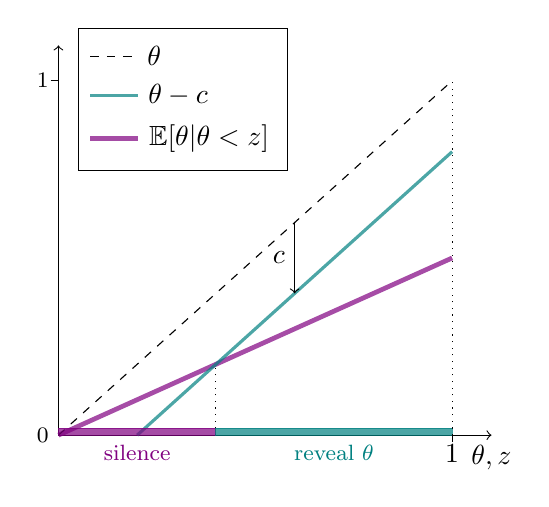
\begin{tikzpicture}[xscale=5,yscale=4.5]
			\draw[->] (0,0) -- (1.1,0) node[below]{$\theta,z$};
			\draw[->] (0,0) -- (0,1.1);
			\draw (0,0) node[left]{\footnotesize $0$};
			
			% Plot
			\draw[line width=0.6mm, violet, opacity=0.7] (0,0) -- (1,0.5);
			\draw[dashed] (0,0) -- (1,1);
			\draw[line width=0.4mm, teal, opacity=0.7] (0.2,0) -- (1,0.8);
			\draw[<-] (0.6,0.4) -- (0.6,0.5) node[left]{$c$} -- (0.6,0.6);
			\draw[dotted] (0.4,0) -- (0.4,0.2);
			
			\filldraw[violet, opacity=0.7] (0,0) -| (0.4,0.02) -| (0,0);
			\draw (0.2,0) node[below, violet]{\footnotesize silence};
			\filldraw[teal, opacity=0.7] (1,0) -| (0.4,0.02) -| (1,0);
			\draw (0.7,0) node[below, teal]{\footnotesize reveal $\theta$};
			
			% Ticks
			% x axis
			\draw (1,0) coordinate(q3) node[below]{$1$};
			\draw (q3) ++(0,-0.02) -- ++(0,0.02);
			\draw[dotted] (1,0) -- (1,1);
			
			% y axis
			\draw (0,1) coordinate(u2) node[left]{\footnotesize $1$};
			\draw (u2) ++(-0.02,0) -- ++(0.02,0);
			%\draw[dotted] (u2) -- (1,1);
			
			%Legend
			\matrix [draw, fill=white, below right] at (0.05,1.15) {
				\draw [dashed] ++(-0.3,0) -- ++(0.6,0) node[black,right] {$\theta$}; \\
				\draw [line width=0.4mm, teal, opacity=0.7] ++(-0.3,0) -- ++(0.6,0) node[black,right, opacity=1] {$\theta-c$}; \\
				\draw [line width=0.6mm, violet, opacity=0.7] ++(-0.3,0) -- ++(0.6,0) node[black,right,opacity=1] {$\mathbb{E}[\theta | \theta<z]$}; \\
			};
		\end{tikzpicture}
	\end{column}
\end{columns}
\end{frame}


\begin{frame}{Uncertain evidence \citep{dye_disclosure_1985,jung_disclosure_1988}}
\begin{itemize}
	\item Now return to the case $c=0$, but the firm only has \structure{evidence with probability $\lambda < 1$}.
	\item With probability $1-\lambda$ the firm has no evidence and is forced to stay silent.
	\item Then, if types $\Theta_S$ stay silent:
	\begin{align*}
		\mathbb{E}[\theta \mid \text{silence}] = \frac{\lambda \mathbb{P}(\Theta_S) \mathbb{E}[\theta \mid \Theta_S] + (1-\lambda) \mathbb{E}[\theta]}{\lambda \mathbb{P}(\Theta_S) + (1-\lambda)} > \mathbb{E}[\theta \mid \Theta_S].
	\end{align*}
	The consumer is not as pessimistic after no disclosure (as when $\lambda=1$), because they understand the firm may not have any evidence. So profit from disclosure is smaller.
	\item This may again lead to some low types staying silent (pretending to have no evidence).
\end{itemize}
\end{frame}


\begin{frame}{Uncertain evidence: example}
\begin{columns}
	\begin{column}{0.6\linewidth}
		{\setstretch{1.3}
			\begin{itemize}
				\item Suppose again $\theta \sim U[0,1]$ and let $\lambda = 3/4$.
				\item In eqm, types $\theta \in [z,1]$ disclose their type if they can; types $\theta \in [0, z)$ always silent (same argument as in costly disclosure). Then using LIE and Bayes' rule,
				\pause
				\begin{align*}
					\mathbb{E}[\theta \mid \text{silence}] 
					%= \frac{\lambda \mathbb{P}(\Theta_S) \mathbb{E}[\theta \mid \theta \in \Theta_S] + (1-\lambda) \mathbb{E}[\theta]}{\lambda \mathbb{P}(\Theta_S) + (1-\lambda)} 
					%= \frac{\frac{3}{4} \cdot z \cdot \frac{x}{2} + \frac{1}{4} \cdot \frac{1}{2}}{\frac{3}{4} \cdot z + \frac{1}{4}} 
					= \frac{3z^2 + 1}{2(3z + 1)}
				\end{align*}
				\item Type $\theta$ discloses if $\theta \geq \mathbb{E}[\theta \mid \text{silence}]$ and silent otherwise. Hence $z = \mathbb{E}[\theta \mid \text{silence}] \iff z =1/3$.
				\item Eqm: types $\theta \in [1/3,1]$ disclose if they can; types $\theta \in [0, 1/3)$ always stay silent.
			\end{itemize}
		}
	\end{column}
	\begin{column}{0.4\linewidth}
		%\pause[1]
		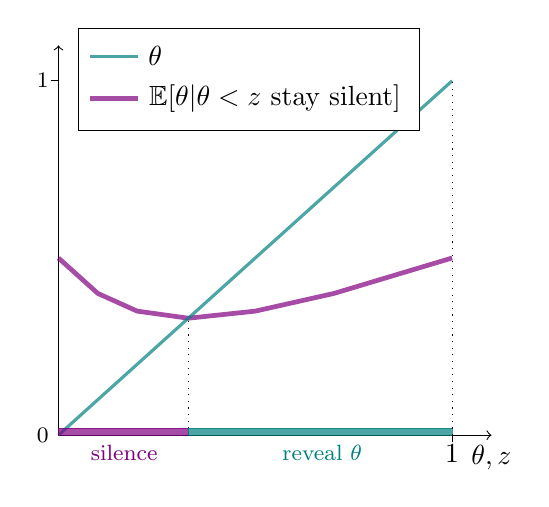
\begin{tikzpicture}[xscale=5,yscale=4.5]
			\draw[->] (0,0) -- (1.1,0) node[below]{$\theta,z $};
			\draw[->] (0,0) -- (0,1.1);
			\draw (0,0) node[left]{\footnotesize $0$};
			
			% Plot
			\draw[line width=0.6mm, violet, opacity=0.7, smooth] (0,0.5) -- (0.1,0.4) -- (0.2,0.35) -- (0.33,0.33) -- (0.5,0.35) -- (0.7,0.4) -- (1,0.5);
			\draw[line width=0.4mm, teal, opacity=0.7] (0,0) -- (1,1);
			\draw[dotted] (0.33,0) -- (0.33,0.33);
			
			\filldraw[violet, opacity=0.7] (0,0) -| (0.33,0.02) -| (0,0);
			\draw (0.167,0) node[below, violet]{\footnotesize silence};
			\filldraw[teal, opacity=0.7] (1,0) -| (0.33,0.02) -| (1,0);
			\draw (0.67,0) node[below, teal]{\footnotesize reveal $\theta$};
			
			% Ticks
			% x axis
			\draw (1,0) coordinate(q3) node[below]{$1$};
			\draw (q3) ++(0,-0.02) -- ++(0,0.02);
			\draw[dotted] (1,0) -- (1,1);
			
			% y axis
			\draw (0,1) coordinate(u2) node[left]{\footnotesize $1$};
			\draw (u2) ++(-0.02,0) -- ++(0.02,0);
			%\draw[dotted] (u2) -- (1,1);
			
			%Legend
			\matrix [draw, fill=white, below right] at (0.05,1.15) {
				\draw [line width=0.4mm, teal, opacity=0.7] ++(-0.3,0) -- ++(0.6,0) node[black,right, opacity=1] {$\theta$}; \\
				\draw [line width=0.6mm, violet, opacity=0.7] ++(-0.3,0) -- ++(0.6,0) node[black,right,opacity=1] {$\mathbb{E}[\theta | \theta < z \text{ stay silent}]$}; \\
			};
		\end{tikzpicture}
	\end{column}
\end{columns}
\end{frame}


\begin{frame}{Naive receiver \citep{milgrom_relying_1986}}
\begin{itemize}
	\item Go back to the base setup, but assume that with probability $\pi \in [0,1]$ the receiver/consumer is \alert{na{\"i}ve} (or, as \cite{eyster_cursed_2005} call them, \alert{cursed}).
	
	\item A cursed receiver makes no inference from silence: $\mathbb{E}[\theta \mid \text{silence} ] = \mathbb{E}[\theta]$; is otherwise same as a rational receiver.
	
	\pause \bigskip 
	\item Then if $\theta \sim [0,1]$ and the firm reveals $\theta$ iff $\theta \geq z$, eqm cutoff $z$ must be such that:
	\begin{align*}
		z = \pi \mathbb{E}[\theta] + (1-\pi) \mathbb{E}[\theta \mid \Theta_S] = \frac{\pi}{2} + (1-\pi)\frac{z}{2}
		&& \Rightarrow &&
		z = \frac{\pi}{1+\pi}.
	\end{align*}
	So in equilibrium, the firm reveals $\theta$ only if $\theta > \frac{\pi}{1+\pi}$ \\
	(i.e., always reveals when $\pi=0$; reveals only if $\theta>\mathbb{E}[\theta]$ when $\pi=1$).
\end{itemize}
\end{frame}


\begin{frame}{Dislosure: Interim conclusion}
\begin{itemize}
	\item In the basic game with evidence, unraveling leads to \structure{full information revelation}.
	\item Unraveling can be tamed in many ways, including disclosure costs, na{\"i}vet{\'e}, or receivers allowing for a chance of sender having no evidence. (There are, of course, not the only reasons; see \cite{dranove_quality_2010} for more.)
	\item Even in those later cases, the idea is simple: \structure{reveal good news}, \alert{hide bad news}.
	\item Think of evidence and incentives to reveal it as an additional tool in your information extraction toolbox.
\end{itemize}
\end{frame}


\begin{frame}{Good news and bad news}
	The asymmetry between \textbf{good \& bad news} is fun to explore:
	\begin{itemize}[<+->]
		\item it means that \alert{silence is bad news} (but humans are bad at inferring it, see \cite*{jin_is_2021}), 
		\item that \alert{silence leaves more uncertainty} than good announcements \citep{shin_disclosures_2003}, 
		\item that bad news are revealed in \alert{bunches} \citep*{acharya_endogenous_2011}
		\item that the desire to have good news to disclose leads to \alert{excessive risk-taking} \citep*{ben-porath_disclosure_2018} %\alert{excessive information acquisition} and 
		
		\bigskip 
		\item There are also a few reasons why sender might want to voluntarily reveal bad news, see an overview in \cite{smirnov_bad_2022}
	\end{itemize}
\end{frame}


%\begin{frame}{A word from our sponsor}
%\begin{itemize}
%	\item As usual, \textbf{dynamic disclosure games} are also extremely fun (with evidence arriving over time and sender choosing what/when to disclose), but we won't talk about those. Instead... 
%\end{itemize}
%\end{frame}


\section{Disclosure with one sender: mechanism design}

\begin{frame}{Evidence and Mechanism design}
\begin{itemize}
	\item We have looked at disclosure games so far, where receiver/designer had to be sequentially rational (maximize $\mathbb{E}u_R$ given $m$ $\Rightarrow$ choose $x=\mathbb{E}[\theta|m]$).
	\item What if we take a mechanism design perspective? I.e., suppose the receiver can \alert{commit} to a decision rule $x(m)$. Can this help produce a \structure{better outcome?}
	\begin{itemize}
		\item E.g., in the \textbf{Dye setting} (uncertain evidence).
		\item Note: choosing a strategy $x(m)$ in the no-commitment game can be seen as ``a mechanism design problem with a sequential rationality constraint''. Extra constraint = worse outcome. Or is it?
	\end{itemize}

	\pause \bigskip 
	\item \citet*{hart_evidence_2017} show this is not the case.
	\item Their result: under some conditions on the sender's evidence and the receiver's preferences (that our setting satisfies): 
	\begin{itemize}
		\item disclosure game has a unique equilibrium,
		\item the optimal disclosure mechanism exists and is unique,
		\item the two \structure{coincide} $\Rightarrow$ \textbf{no value from commitment}.
	\end{itemize}
\end{itemize}
\end{frame}


\begin{frame}{Evidence and Mechanism design 2}
\begin{itemize}
	\item Their result (no value from commitment) relies on concavity of the receiver's preferences + assumptions on evidence structure. 
	\item \textbf{Counterexample} with preferences not concave in $x$ given $\theta$:
	\item Let $\theta \in \{1,2,...,999\}$ with $\phi_0(999) = 0.002$ and $\phi_0(\theta) = 0.001$ for $\theta < 999$.
	\item Suppose types $\theta<999$ are verifiable: $m \in \{\varnothing, \theta\}$; type $\theta=999$ has no evidence: $m = \varnothing$.
	\item Receiver's payoff is $u_R(x,\theta) = \mathbb{I}\{x=\theta\}$; sender's payoff is still $u_S(x,\theta)=x$.
	\pause \bigskip 
	\item Then commitment outcome is better than no commitment:
	\begin{itemize}
		\item In eqm w/o commitment, after silence the receiver chooses $x(\varnothing)=999$, so sender never reveals $\theta$. $\Rightarrow \, \mathbb{E}u_R = 0.002$.
		\item With commitment, receiver can commit to $x(\varnothing)=1$ $\Rightarrow$ sender reveals $\theta$ if possible $\Rightarrow$ $\mathbb{E}u_R = 0.998$.
	\end{itemize}
\end{itemize}
\end{frame}


\section{Disclosure with many senders}

\begin{frame}{Many senders, same evidence \citep{milgrom_relying_1986}}
\begin{itemize}
	\item Go back to the game with \textbf{na{\"i}ve receiver}, but suppose that in addition to \structure{the firm}, there is now also \alert{a competitor}.
	\item Both observe firm quality $\theta$ and can disclose it in a verifiable way.
	\item The competitor's payoff is $-\mathbb{E}[\theta|\phi_c]$, the opposite of the firm's.
	
	\pause\bigskip 
	\item Then the firm wants to reveal $\theta$ iff $\theta > \pi \mathbb{E}[\theta] + (1-\pi) \mathbb{E}[\theta \mid \text{silence}]$.
	\item Similarly, the competitor wants to reveal $\theta$ iff $\theta < \pi \mathbb{E}[\theta] + (1-\pi) \mathbb{E}[\theta \mid \text{silence}]$.
	\item Regardless of $\theta$, one of them wants to reveal $\Rightarrow$ someone always reveals $\theta$ \\
	$\Rightarrow$ \structure{full info} in equilibrium.
\end{itemize}
\end{frame}


\begin{frame}{Many senders, same evidence}
\begin{itemize}
	\item Conclusion: if players have a \alert{conflict of interest} and access to the same info, \alert{more information} is revealed. 
	
	\item This complements the results without evidence: the receiver can exploit the conflict of interest between players to extract more info (we saw this in the \cite{battaglini_multiple_2002} model).
\end{itemize}
\end{frame}


\begin{frame}{Item allocation with evidence \citep*{ben-porath_mechanisms_2019}}
\begin{itemize}
	\item Evidence+competition help elicit info even with no common info.
	\item E.g., consider an \textbf{item allocation problem:} 
	\begin{itemize}
		\item $N$ bidders with private, \alert{verifiable} types $\theta_i$; designer chooses allocation $x \in \varDelta(N)$;
		\item $u_i(x,\theta) = x_i \theta_i$;
		%\mathbb{I}\{x_i=1\}$ ($i$ benefits from getting the item, but $\theta_i$ is not $i$'s valuation)
		\item $u_0(x,\theta) = \sum_{i=1}^N x_i \theta_i$ (designer wants to allocate to highest $\theta_i$).
	\end{itemize}
\end{itemize}
\end{frame}


\begin{frame}{Item allocation with evidence}
\begin{itemize}
	\item \textbf{Without evidence,} we'd have to require payments as a proof of high $\theta_i$.
	\item \textbf{With evidence,} can simply ask a player to show proof of their high $\theta_i$ 
	\\ $\Rightarrow$ efficient allocation is implementable even without transfers!
	%\begin{itemize}
	%	\item Words in Dye setting (uncertain evidence) too
	%\end{itemize}
	\item The same is true even if \alert{$u_i(x,\theta) = \mathbb{I}\{x_i=1\}$}
	\begin{itemize}
		\item i.e., if players don't care about their $\theta_i$, only the principal does
		\item no single-crossing in this case $\Rightarrow$ transfers wouldn't implement the principal's desired allocation
		\item Example: investor only wants to fund projects that are genuinely good, but all entrepreneurs think their projects are genuinely good
	\end{itemize}
	\pause \bigskip 
	\item Bottom line: 
	\begin{itemize}
		\item Evidence helps info elicitation
		\item Evidence makes commitment power unnecessary
	\end{itemize}
	%\item Their results:
	%\begin{enumerate}
	%	\item \textbf{Commitment has no value to the principal!}
	%	\item Randomization has no value for the principal!
	%	\item DSIC=BIC (=Robust IC, stronger than DSIC)
	%\end{enumerate} 
\end{itemize}
\end{frame}


\begin{frame}{Evidence: Conclusion}
\begin{itemize}
	\item \structure{Evidence helps info elicitation}, and may even lead to unraveling of all of players' private info
	\item Some factors (like direct cost of disclosure or a milder penalty for silence) may \alert{hinder disclosure}; \structure{competition stimulates} it.
	\item The intrinsic incentives to disclose evidence may be strong enough to render \structure{commitment useless} for the principal/receiver
	\begin{itemize}
		\item Good news for receiver -- can achieve commitment outcome even without any commitment power!
	\end{itemize}
\end{itemize}
\end{frame}


\appendix
\begin{frame}[allowframebreaks]{References}
\bibliography{teaching}
\bibliographystyle{abbrvnat}
\end{frame}


\end{document}